\documentclass[onecolumn, draftclsnofoot,10pt, compsoc]{IEEEtran}
\hbadness=1000 % suppress warnings
\usepackage{graphicx}
\usepackage{url}
\usepackage{setspace}
\usepackage{hyperref}
\usepackage{listings}
\usepackage{cite}
\usepackage{geometry}

\usepackage{longtable}

\geometry{textheight=9.5in, textwidth=7in}

% 1. Fill in these details
\def \CapstoneTeamName{		Aerolyzer}
\def \CapstoneTeamNumber{		19}
\def \GroupMemberOne{			Daniel Ross}
\def \GroupMemberTwo{			Kin-Ho Lam}
\def \GroupMemberThree{			Logan Wingard}
\def \CapstoneProjectName{		Aerolyzer}
\def \CapstoneSponsorCompany{	NASA JPL}
\def \CapstoneSponsorPerson{		Kim Whitehall}


% 2. Uncomment the appropriate line below so that the document type works
\def \DocType{		%Problem Statement
	%Requirements Document
	%Technology Review
	%Design Document
	Progress Report
}

\newcommand{\NameSigPair}[1]{\par
	\makebox[2.75in][r]{#1} \hfil 	\makebox[3.25in]{\makebox[2.25in]{\hrulefill} \hfill		\makebox[.75in]{\hrulefill}}
	\par\vspace{-12pt} \textit{\tiny\noindent
		\makebox[2.75in]{} \hfil		\makebox[3.25in]{\makebox[2.25in][r]{Signature} \hfill	\makebox[.75in][r]{Date}}}}
% 3. If the document is not to be signed, uncomment the RENEWcommand below
\renewcommand{\NameSigPair}[1]{#1}

%%%%%%%%%%%%%%%%%%%%%%%%%%%%%%%%%%%%%%%
\graphicspath{{images/}}
\begin{document}
	\begin{titlepage}
		\pagenumbering{gobble}
		\begin{singlespace}
			\centering
			
\includegraphics[height=4cm,natwidth=345,natheight=435]{images/coe_v_spot1.png}
			\hfill 
			% 4. If you have a logo, use this includegraphics command to put it on the coversheet.
			%\includegraphics[height=4cm]{CompanyLogo}   
			\par\vspace{.2in}
			\centering
			\scshape{
				\huge CS Capstone \DocType \par
				{\large\today}\par
				\vspace{.5in}
				\textbf{\Huge\CapstoneProjectName}\par
				\vfill
				{\large Prepared for}\par
				\Huge \CapstoneSponsorCompany\par
				\vspace{5pt}
				{\Large\NameSigPair{\CapstoneSponsorPerson}\par}
				{\large Prepared by }\par
				Group\CapstoneTeamNumber\par
				% 5. comment out the line below this one if you do not wish to name your team
				\CapstoneTeamName\par 
				\vspace{5pt}
				{\large
					\NameSigPair{\GroupMemberOne}\par
					\NameSigPair{\GroupMemberTwo}\par
					\NameSigPair{\GroupMemberThree}\par
				}
				\vspace{20pt}
			}
			\begin{abstract}  
				The Aerolyzer Project aims to deliver a new source of air quality and weather information through leveraging existing weather data and image analysis algorithms.
				When complete, this open-source project shall feature a Python library that uses image classification and third-party weather APIs, displayed with an intuitive web-based user interface.
				This document outlines the software design descriptions for the Aerolyzer Library. 
			\end{abstract}     
		\end{singlespace}
	\end{titlepage}
\section{Table of Contents}
\tableofcontents
\bibliographystyle{IEEEtran}
\bibliography{ref}
\clearpage

\begin{singlespace}

	\section{Project Purpose}
		Monitoring atmospheric aerosols is important due to their effects on the atmosphere's chemical composition and radiation distribution.
		The presence of aerosols reduces air quality which can potentially lead to health complications such as bronchitis or respiratory inflammation.
		Unfortunately, aerosols in the atmosphere are constantly changing, and current satellite, aircraft, and ground-based instruments do not simplify data enough for the average person to understand.
		There is currently no way to judge local air quality using regional aerosol data without in-depth atmospheric knowledge.
		Additionally, delayed or inaccurate atmospheric reports complicate getting reliable local atmospheric information.


		The primary objective of the Aerolyzer project is to create a tool that infers local air quality using regional weather data and aerosol analysis.
		To accomplish this goal, the Aerolyzer project requires a Python library that identifies images relevant to aerosols, analyzes acceptable images for aerosol content, stores relevant information for trend analysis, and compiles weather information with its aerosol data.
		
	\section{Current State}
		As of December, Kin-Ho has designed and tested two horizon detection classifiers using OpenCV 3.3.0.
		Ongoing work on the project can be viewed in the Aerolyzer library’s open-source Github.
		These classifiers are horizon detection by straight line and horizon detection by color threshold.

	\section{Issues - Kin-Ho Lam}
		My understanding of committing to Github in accordance with Apache open-source standards is lacking.
		Although I believe the state of our project is pretty far ahead in terms of development, I am struggling to meet our client's expectations of clean github commits.
		My solution to this issue is to research and practice Apache open-source principals throughout winter break.
		I am committed to the success of this project and I want to ensure my contributions adhere to the standards set by Dr. Whitehall.

	\section{Retrospective}
		\subsection{Kin-Ho Lam}
		\begin{longtable}{|l|p{0.3\linewidth}|p{0.3\linewidth}|p{0.3\linewidth}|}\hline \textbf{Week} & \textbf{Positives} & \textbf{Deltas} & \textbf{Actions}\\\hline
		1 	& This week we submitted our project preferences. & - & -\\\hline

		2 	&
			We received our group and project assignments. I sent an introductory email to Dr. Whitehall introducing myself, teammates, and established points of contact.
			We video conferenced with Dr. Whitehall on Friday, 10/6/17.
			During this meeting Dr. Whitehall introduced herself and talked about the goals of the project.
			She also discussed the Apache open-source nature of the project.
			Over the weekend Logan, Daniel, and I met to review the past team's work.
			&
			We need to establish a project work-flows, namely understand what tools we can leverage to accomplish our project's goals. 
			&
			I intend to build a development virtual machine to standardize development environments.
			This VM shall contain all libraries necessary to develop the Aerolyzer Python library.
			\\\hline

		3	&
			Logan, Daniel, and I discussed the previous group's progress.
			In our Weekly meeting with Dr. Whitehall, we discussed a standardized VM environment.
			She prefers a cloud-based development environment, but was OK with me creating one for experimentation.
			&
			We don't understand why this project has moved to a release stage, why does it have a functioning website when there is no aerosol analysis back-end?
			&
			It's not my job to ask questions, I just want to contribute to the project.
			I created a Linux development environment and uploaded it to the group's shared Google Drive space.
			This VM consists of Ubuntu 16.04 and has Python 2.7.1, OpenCV 3.3.0 and all necessary required libraries pre-installed.
			\\\hline

		4	&
			We wrote and submitted a draft of our problem statement to Dr. Whitehall.
			&
			While she didn't seem to comment on the quality of the writing, I believe this initial draft was very lacking in terms of structure, grammar, and clarity.
			&
			I outlined the following guidelines I'd like to see changed in this document:
			\begin{itemize}
				\item Write this document in such a way that a person who has no knowledge of atmospheric Aerosols can understand our project.
				\item Be specific about the terms we define.
				\item Organize this document in a clear way where we introduce new information and build on it.
			\end{itemize}
			\\\hline

		5 	&
			We continued to discuss the github workflow and tools we're going to used.
			I wanted to use sort of an "agile whiteboard" to discuss project roles and tasks, Kim preferred we use the Github issues.
			I outlined a plan of the classifier driver.
			&
			We need a working plan for our classifier design.
			The old team's pseudo-code isn't very useful, they assume color histograms generated by OpenCV give more information than they actually do.
			I believe the most effective horizon filter will combine the use of supervised and unsupervised learning.
			&
			We plan to use 2 classifiers, one to detect horizons, another to detect the presence of a sunrise or sunset.
			The horizon classifier exists because you logically can't have a sunrise or sunset without a horizon.
			\\\hline

		6	&
			This week we discussed machine learning libraries we could use with our TA.
			He stated that more research is needed, if we want to use a supervised learning library then we need some way to get a very large dataset.
			&
			We currently do not have a large reliable dataset to train a future supervised learning library.
			&
			I assigned Daniel to look into scraping instagram and google images for the \#sunrise / \#sunset / \#nofilter tags.
			\\\hline

		7	&
			I created the Horizon Detection by Straight Line algorithm.
			Further details on this algorithm can be found below.
			&
			Kim stated her discontent with how we were treating the Git workflow.
			&
			I need to understand and research further to gather what I'm doing wrong and fix it.
			Main objectives include making sure she's informed about what we're doing. 
			We need to communicate over channels she looks at, so through email and cc'ing her, Github issues, or slack channels.
			\\\hline

		8	&
			We are stressing to complete the Technology Review Document.
			We moved our meeting with Kim to Tuesday, the 28th to avoid finals week.
			&
			Issues with Github are ongoing, we need to work harder on trying to understand what she needs.
			&
			Logan is having a 1-1 session with Kim to talk about how to use Github. I'll do research on my own and ask Logan what he learned.
			\\\hline

		9	&
			I created the Horizon Detection by Threshold algorithm.
			This new approach uses a binary threshold to separate the sky from the foreground.
			Further details can be found below.
			&
			Kim was not happy with the large amount of data I had in my pull request.
			&
			I removed the test images I used and moved them to the shared Google drive.
			I also squashed my commits.
			\\\hline

		10	&
			We are struggling to finish the design document and compile all our notes.
			I have managed to solve a few compile errors in our Progress Report and Design document.
			We submitted all documents by midnight.
			&
			Latex was giving us a bit of a hard time, I stopped writing in overleaf and started following the errors it was giving us.

			\\\hline
		\end{longtable}
		\subsection{Logan Wingard}
		\begin{longtable}{|l|p{0.3\linewidth}|p{0.3\linewidth}|p{0.3\linewidth}|}\hline \textbf{Week} & \textbf{Positives} & \textbf{Deltas} & \textbf{Actions}\\\hline
		1 	& We chose our top 5 projects. & All of the projects I selected were taken. Five more project preferences need to be submitted. & I sent in my additional five project preferences. \\\hline

		2 	& We met with Kim Whitehall, the client for our chosen project "Aerolyzer". & We must write our individual problem statements. The problem statement should clearly describe the problem that Aerolyzer will solve, the proposed solution (how we plan to solve the problem), and performance metrics, which includes definitions and accuracy specifics.  & We met with Kim Whitehall and were able to get an understanding of the problem we are trying to solve using Aerolyzer. I used this information to write and submit my individual problem statement. \\\hline

		3 	& I recieved a lot of feedback on my individual problem statement. We met with our TA for the first time this week and learned what is being looked for in the complete team problem statement, as well as the requirements doc.  & Much of my problem statement needs to change before we can compile all the problem statements into one. & I made edits to my problem statement and we started the compilation process. \\\hline

		4 	& We completed our problem statement and submitted it. Kin-Ho was able to set up a virtual machine to use as a development environment.  & Boundaries need to be set in our group after high tensions lead to some unwanted surprises. We also need to start writing the requirements document. & We submitted the problem statement and tensions have lowered. We spoke with the TA and got some instructions for the requirements document. \\\hline

		5 	& Submitted the requirements document rough draft. & Rough draft is missing a ghant chart. We need to make and include a ghant chart into our requirements doc before we submit the final. We need to configure the library so that the functions we write are imported along with Aeorlyzer. & We submitted the rough draft of the requirements document. I researched a bit into creating modules in python. \\\hline

		6 	& Daniel created a very nice ghant chart to go in the requirements document and the final draft is looking great. & We've been looking into horizon detection in OpenCV and found a python script online. We are going to modify it to see if it would work in our context, and if it does, we will contact the writer to ask permission to use it. & After tinkering with the code we found, we determined it does not meet our needs and we will not be contacting the creator of it. \\\hline

		7 	& Succesfully setup the python module on the virtual machine. & I need to look into the setup.py file and determine what needs to be done to ensure anyone who imports aerolyzer from Pypi has access to all the functions we have been writing. & I've been researching python's package index and understanding the syntax needed in the setup.py file to ensure Aerolyzer has what it needs to run our functions. \\\hline

		8 	& Set a meeting with Kim Whitehall to help me understand git and github better. & I've been pushing my work to the wrong fork and need to get git straightened out. & I've arranged a meeting with Kim to ensure that I understand git and our project's workflow. I also forked the repo and created, then removed, a test file and made a pull request as practice. \\\hline

		9 	& I had my meeting with Kim about git and it all makes much more sense to me. I found the meeting extremely helpful. & We need to work on the Technology review document. & Been working on the Tech review. putting a lot of research time into neural networks, image scrapers and library structures. \\\hline

		10 	& Fixed many of the errors in my section of the Tech review thanks to helpful feedback from Winters. & The design document needs to get started and submitted by Friday. We are also now having problems with the google drive and are unable to upload files to the drive. & We've been putting a lot of time into the design document and have been struggling a lot with the LateX syntax. After troubleshooting the LateX file for a bit, we succesfully got it to compile how we liked it and submitted it to our Onenote and emailed it to Winters. \\\hline
		\end{longtable}


		

	\section{Horizon Detection Filter}
      \subsection{Design Elements - OpenCV \& Google Tensorflow}
      		\subsubsection{Design Attributes}
		        Outlined in the Software Design Document, a horizon detection filter shall be created using OpenCV and other python libraries as required.
				OpenCV is a BSD-licensed computer-vision library with many relevant sub-modules.
				Containing over 2,500 algorithms, OpenCV can analyze images and videos, recognize faces, identify objects, perform visual transformations, and more.
				One can use image transformations to normalize image data such that a classifier can more easily distinguish what is in a given image.
				\cite{svm}

				An advanced machine learning library, Google Tensorflow can build versatile and accurate predictive data models provided a large dataset of training images.
				One can apply Tensorflow to the Aerolyzer project by training its inception module to recognize patterns in a large dataset consisting of acceptable images of the horizon.
				A human will need manually pre-classify and build a test dataset consisting of acceptable images. \ref{acc_img}
				Tensorflow’s ease of use, proven library, and ample documentation makes it a potential candidate to create a powerful image classifier. \cite{rhnvrm} \cite{RNN}

          \subsubsection{Design Relationships}
					.\\
					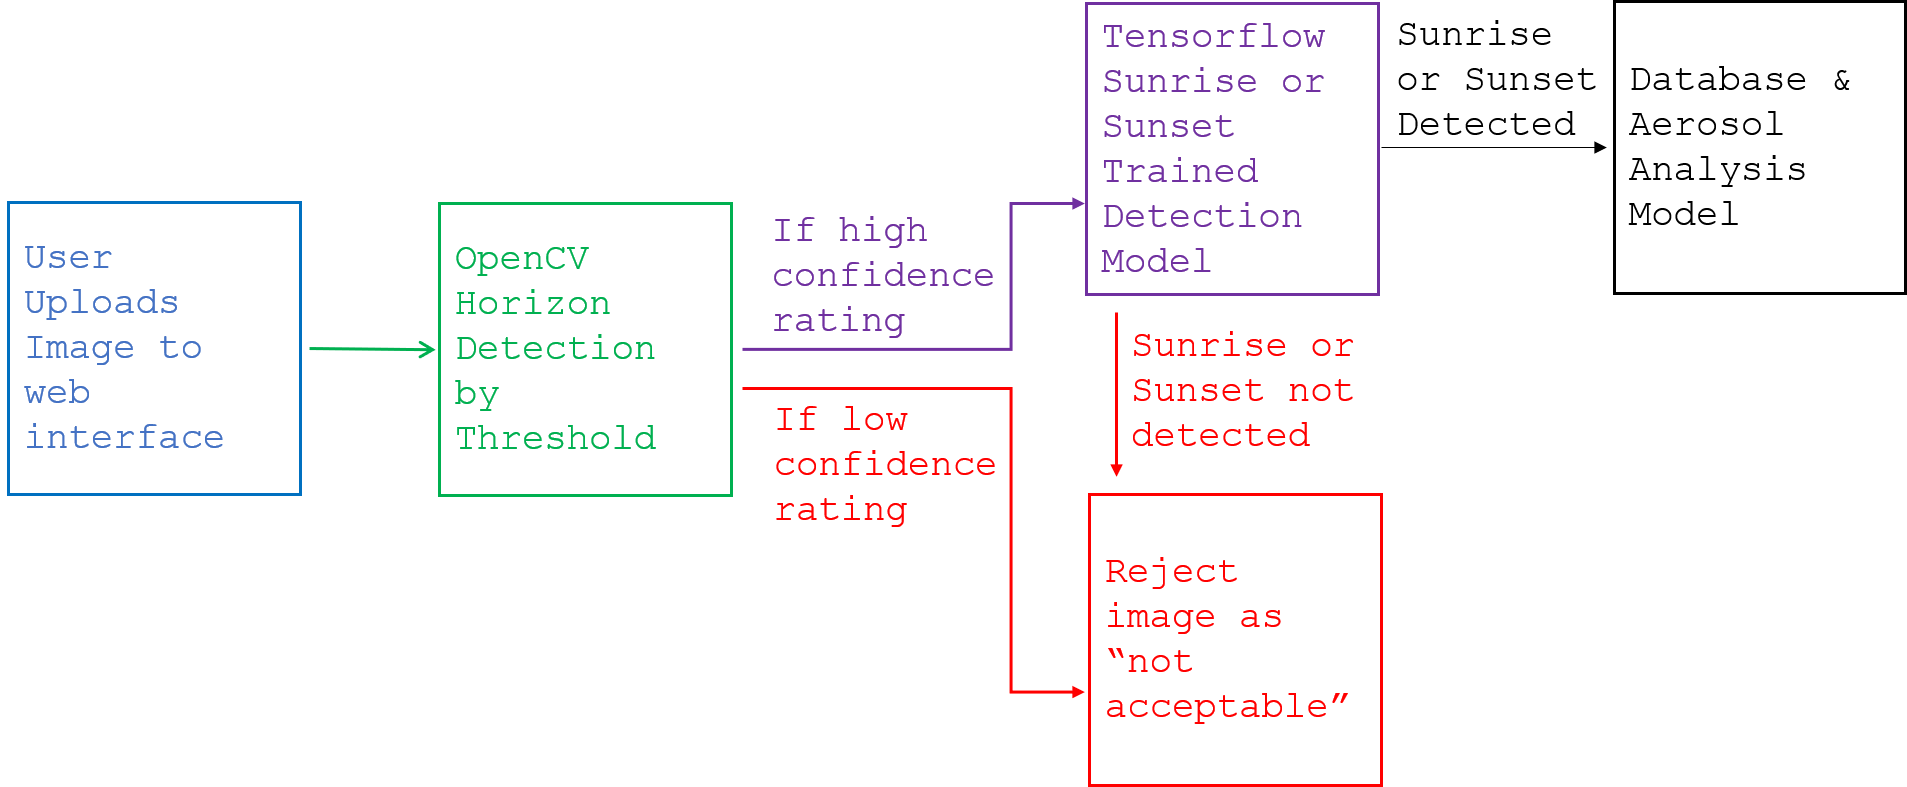
\includegraphics[width=4.5in,natwidth=1907,natheight=787]{images/tensor.png}

		\subsubsection{Design Constraints}
			Aerolyzer’s unique image criterion necessitates a predictive data model capable of detecting horizons with a minimum of 66\% certainty and sunsets or sunrises with a minimum of 50\% certainty.
			Efficient and expedient algorithm performance is necessary due to the expected user base who will be waiting for Aerolyzer to service their request.
			Pending further research, these criterion are achievable through OpenCV and Tensorflow.
			More computer vision libraries or modules may be required.
	      
		\subsubsection{OpenCV Horizon Detection by Straight Line Algorithm}
			Horizon detection by straight line seeks to detect the simplest possible acceptable image; a picture of the sunset/sunrise without obstructions.
			In this case, one can expect the most visible longest and straightest line in an image to be the horizon.
			With this assumption, the Horizon Detection by Straight Line algorithm shall accept or reject an image through the following procedure:
			\begin{enumerate}
				\item Upon receiving an image, detect the longest and straightest line.
				\item If there is no straight line stretching across the image, reject it.
			\end{enumerate}
			As a proof of concept, the algorithm is implemented in the following python function.
			This algorithm draws a straight green line where it believes the horizon is.
			\lstinputlisting[language=Python,basicstyle=small]{code/HorizonDetectionbyStraightLine.py}

			Upon image submission, the Horizon Detection by Straight Line’s algorithm works as follows:
				
				\begin{enumerate}
					\item Perform a gaussian blur on the image
					\item Convert the image to grayscale
					\item Perform Canny Edge Detection \cite{svm}
					\item Perform Hough Line Transformation \cite{svm}
					\item If there is a straight line, draw a green line spanning across the image.
						This is the classified horizon.
					\item Else, if there are no straight lines, then reject the image.
				\end{enumerate}


				This approach works well for some images such as fig X pulled from the Aerolyzer test image album.
		However, it is clear that this approach does not work for all cases, as seen in fig Y, detecting the horizon by straight line fails in images with a complex foreground that contains many straight lines.
		A new algorithm is necessary to enhance detection accuracy.
				\\
				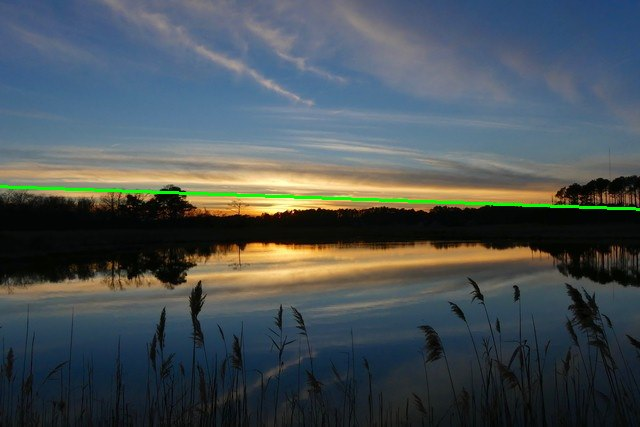
\includegraphics[width=4.5in,natwidth=640,natheight=427]{images/line1.jpg}
				\\
 				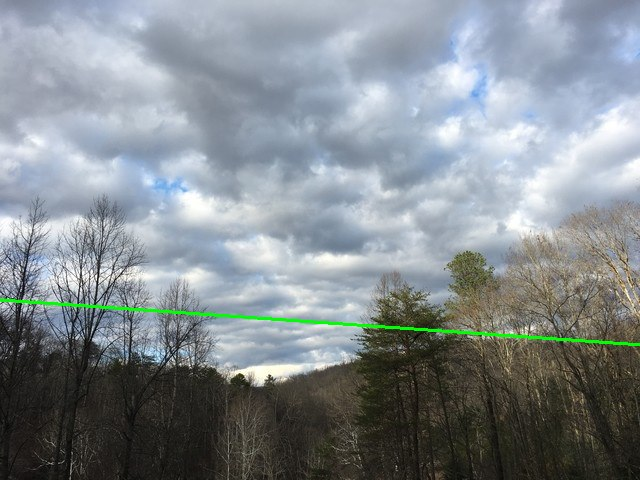
\includegraphics[width=4.5in,natwidth=640,natheight=480]{images/line2.jpg}

				\subsubsection{OpenCV Horizon Detection by Threshold}
						Horizon Detection by Threshold is a more versatile method compared to straight line detection because it relies on segmenting color distribution.
					Detection by Threshold was designed to classify images that contain complex foregrounds by distinguishing what part of the image is the sky.
					The Threshold algorithm shall accept or reject an image through the following procedure:
					\begin{enumerate}
						\item Separate the image by distinct color spaces
						\item Perform a binary threshold with the minimum color threshold being the color of the sky.
						\item Calculate the area of the largest continuous contour that is within the sky color threshold.
						\item Apply a statistical function to ratio the area of sky color over the total area of the image to produce a confidence rating.
								A high confidence rating shall indicate that the image contains a horizon while a low confidence rating indicates there is no horizon.
					\end{enumerate}

					As a proof of concept, the algorithm is implemented in the following python function.
					This algorithm draws a green outline of what it believes to be the sky.
					If no contours can be drawn, the algorithm fails the image, meaning no sky or horizon can be detected.\\

					\lstinputlisting[language=Python]{code/HorizonDetectionbyThreshold.py}
							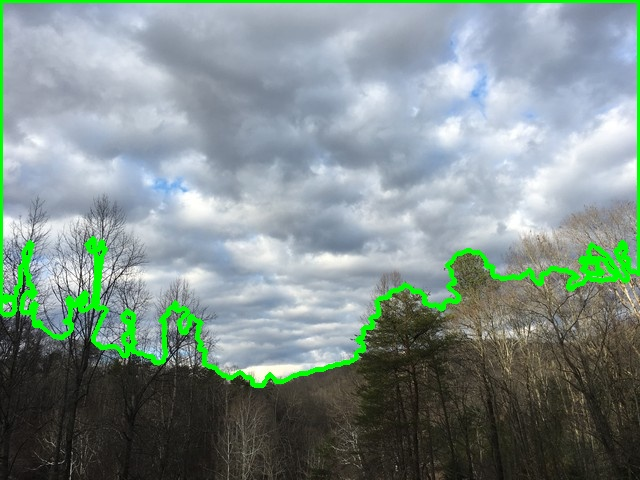
\includegraphics[width=4.5in,natwidth=640,natheight=480]{images/threshold/9.jpg}
					\end{enumerate}
					This algorithm struggles to classify low-light images, improvements and fine-tuning are necessary.

      \subsubsection{Design Rationale}
      	The Aerolyzer Horizon Detection Filter needs to identify acceptable images, namely ones of the sunset or sunrise.
		Research indicates that specific sunset or sunrise image classification  necessitates a predictive Tensorflow model because creating such an unsupervised classifier in OpenCV is a challenging task.
		As demonstrated in Fig.
		Z, this design rationale is accomplished by incorporating a trained Tensorflow model as a secondary step after OpenCV Horizon Detection by Threshold.
		Tensorflow analysis is a computationally expensive process.
		An OpenCV classifier to detect the presence of the sky saves computation time by rejecting all images that do not have skies.
		If no sky is present then it logically follows that there can be no sunrise or sunset in the image.

      \subsubsection{Design languages}
      	An element in the greater Aerolizer python library, the horizon detection algorithm shall be written in Python 2.7.12 while importing OpenCV 3.3.0 and Numpy 1.13.3.
		The Aerolyzer project’s sponsor, Dr.
		Whitehall, chose Python as the library’s primary language.
		

\end{singlespace}
\end{document}
